\input{permve-ntnu-latex-assignment.tex}

\usepackage{float}

\title{	
\normalfont \normalsize 
\textsc{Norwegian University of Science and Technology\\IT3105 -- Artificial Intelligence Programming}
\horrule{0.5pt} \\[0.4cm]
\huge Module 4:\\ Using Minimax with\\ Alpha-Beta Pruning to play 2048\\
\horrule{2pt} \\[0.5cm]
}

\author{Per Magnus Veierland\\permve@stud.ntnu.no}

\date{\normalsize\today}

\begin{document}

\fancyfoot[C]{}
\maketitle

\newpage
\fancyfoot[C]{\thepage~of~\pageref{LastPage}} % Page numbering for right footer
\setcounter{page}{1}

\section*{Branching factor}

The aim of module~4 is to achieve a winning score in the game \textsc{2048}. The game consists of a two-dimensional $4\times 4$ grid where each tile in the grid is either empty or has a number between $2^1$ and $2^{17}$ (inclusive). An upper bound of the game's branching factor can be found by multiplying the number of possible player moves~(4) by the maximum number of empty tiles~(16) by the number of possible tile spawns~(2):

\begin{displaymath}
b_{\textit{upper}} = 4 \cdot 16 \cdot 2 = 128
\end{displaymath}

\section*{State representation}

Given such a large branching factor for each player move it is evident that a large number of states must be evaluated to perform even a shallow search involving a low number of moves. To enable a large number of states to be considered an efficient state representation scheme is beneficial.

Even if the theoretical maximum tile is $2^{17}$, the largest tile required to win the game, 2048, is only $2^{11}$. Given that the number 1 is not present in the game, it is possible to represent the empty tile and tiles for powers of two between $2^1$ and $2^{15}$ by using 4~bits to represent each tile. With 4~bits reserved for each tile, all 16~tiles can be represented by a single 64-bit integer. Using a commonly available 64-bit processor architecture, each board state can be held in a single CPU register.

The resulting representation with example values is shown in Figure~\ref{figure:represent} showing tile values and the corresponding bit values.

\begin{figure}[H]
\centering
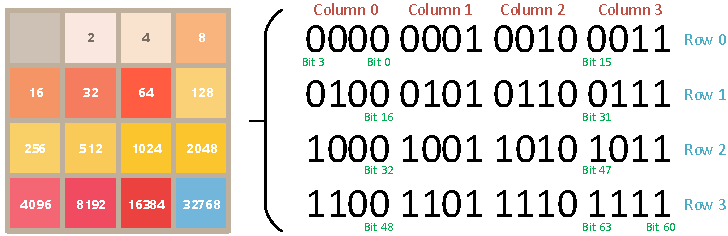
\includegraphics[scale=1.0]{images/2048_state}
\caption{64-bit integer state representation}
\label{figure:represent}
\end{figure}

\section*{Lookup tables}

Another benefit from the compact state representation is that it allows for efficient use of lookup tables. The logic necessary to compute the successor state when given a move requires loops and branches. The effect of performing a move is also local to each row or column, depending on the direction of the move. Each row or column can then be considered in isolation and depend on the exact same logic to produce their successor. The number of possible rows or columns is $2^{16}=65536$, so representing a lookup table for a single direction will take $2^{16}*8=524288$~bytes, or $0.52$~MB. By using four lookup tables, one for each direction, successor states can be evaluated by performing four lookups, one for each row or column.

Lookup tables can also be used to evaluate both board heuristics and board scores. The board heuristic may be a costly function to evaluate, making it very beneficial to pre-compute. However, unlike the state transitions which can be considered as functions considering each row and column individually, the heuristic function evaluates the entire board state. Since a lookup table containing entries for all states would be $2^{64}*8=18.45$~exabytes, this is currently infeasible. However by imposing the limitation that the heuristic function can only consider a single row or column at a time, only a single lookup table with $2^{16}$ entries is needed. This limits the information available to the heuristic function, but the implemented heuristic function is still able to provide sufficient guidance to the search. When evaluating the heuristic value for a state; 8~lookups are performed, one for each row and column, and the result is summed. The advantage of this approach is that the heuristic evaluation can use very costly operations in the pre-computation, since its effective use consists only of lookups.

Evaluating the score of a given state is also done using lookup tables. This is a simple convenience such that the scoring of a state can be performed using four row lookups.

\section*{Expectimax}

The algorithm used to solve \textsc{2048} is \textit{Expectimax} with pruning based on a probability threshold and a transposition table. \textit{Expectimax} was chosen over \textit{Minimax} since the ``adversary'' is stochastic and not actively minimizing the expected outcome. The code centers around the two functions \texttt{score\_player\_node} and \texttt{score\_chance\_node} which calls each other recursively with successive board evaluations, until either the search is pruned due to the node having a probability beneath the probability threshold, or because the depth exceeds the depth threshold, or if the current board state is found in the transposition table.

When traversing downwards into the search, the current probability is tracked such that nodes falling beneath a probability threshold is pruned and heuristically evaluated instead of diving further down their state space. This is done to avoid spending time evaluating unlikely cases, such as when a $4$-tile spawns three times in a row. Using pruning based on probability is very effective, and the pruning rate can typically be 60-80\% without harming the effectiveness of the algorithm.

In addition to pruning based on probability, a configurable depth limit is also imposed to control the algorithm.

When evaluating the game state space, there will be many overlaps where different moves and/or different chance scenarios will end up resulting in the same game state. To improve the algorithm, a transposition table is used where evaluated states in chance nodes are added with their score and depth to a transposition table. If later on, a node is evaluated with a board state which exists in the transposition table, and where the stored depth is greater or equal to the current depth of the new search node, meaning that the current node's state has been evaluated at least as deep as what what the current search would do; the existing score stored in the transposition table is used instead of evaluating the node's state space again. The transposition table typically has a hit rate of 60-70\%.

\section*{Heuristic}

The \textit{Expectimax} algorithm requires a heuristic to evaluate the quality of a given state as it is unfeasible to fully evaluate the full state space for a given node due to a high branching ratio and a typical ``win'' state after approximately 2000~plies.

The chosen heuristic depends on four metrics and six constants. Since a lookup approach is used with the heuristic, the heuristic function can only evaluate a single row or column in isolation. For a given row the number of direct merges, $M_1$, secondary merges, $M_2$, and ternary merges, $M_3$, are recorded. E.g. for a row ``2 2 4 8'' the number of direct merges possible is one (``2'' with ``2'' resulting in ``4''), and the number of secondary merges is one (the resulting ``4'' with the existing ``4'', resulting in ``8''). The number of ternary merges is one (the resulting ``8'' with the existing ``8''). The last metric tracked is the number of ``bad tiles''; $B$. This is simply all non-zero tiles in a row which are not part of a merge.

The first constant, $k_L$, is a base used to distinguish losing states from non-losing states. Since losing states, i.e. states where there are no possible moves, are evaluated to zero -- the heuristic should result in a positive number for any non-losing state.

The three next constants is used to value the different merges, while the constants $k_{B1}$ and $k_{B2}$ is used to adjust the value of ``bad tiles''. A base constant is raised to the power of the number of bad tiles; penalizing each additional ``bad tile'' increasingly.

\begin{displaymath}
H(\textit{row}) = k_L + k_1 \cdot M_1 + k_2 \cdot M_2 + k_3 \cdot M_3 - \frac{{k_{B1}}^{B}}{k_{B2}}
\end{displaymath}

More sophisticated heuristics can be constructed which takes into account the monotonicity of the board state, the values of the tiles involved, and the number of empty tiles. However, the implemented heuristic performs well for shallow depths and is able to achieve a ``2048'' tile on ~80\% of runs with a maximum depth of 4 in under 3 minutes. It also regularly accomplishes the ``4096'' tile; but has not been able to score ``8196'', despite attempts with a maximum depth of 10.

The following constants have been found by thought, trial and error. Achieving good constants for the heuristic will likely involve a meta-search using e.g. a gradient descent approach to tune the algorithm.

\begin{displaymath}
k_L = 100, k_1 = 10, k_2 = 5, k_3 = 2.5, k_{B1} = 5, k_{B2} = 0.08
\end{displaymath}

\end{document}

